\documentclass[11pt,]{article}
\usepackage{lmodern}
\usepackage{amssymb,amsmath}
\usepackage{ifxetex,ifluatex}
\usepackage{fixltx2e} % provides \textsubscript
\ifnum 0\ifxetex 1\fi\ifluatex 1\fi=0 % if pdftex
  \usepackage[T1]{fontenc}
  \usepackage[utf8]{inputenc}
\else % if luatex or xelatex
  \ifxetex
    \usepackage{mathspec}
  \else
    \usepackage{fontspec}
  \fi
  \defaultfontfeatures{Ligatures=TeX,Scale=MatchLowercase}
    \setmainfont[]{Arial}
\fi
% use upquote if available, for straight quotes in verbatim environments
\IfFileExists{upquote.sty}{\usepackage{upquote}}{}
% use microtype if available
\IfFileExists{microtype.sty}{%
\usepackage{microtype}
\UseMicrotypeSet[protrusion]{basicmath} % disable protrusion for tt fonts
}{}
\usepackage[margin=.5in]{geometry}
\usepackage{hyperref}
\hypersetup{unicode=true,
            pdfborder={0 0 0},
            breaklinks=true}
\urlstyle{same}  % don't use monospace font for urls
\usepackage{natbib}
\bibliographystyle{plainnat}
\setlength{\emergencystretch}{3em}  % prevent overfull lines
\providecommand{\tightlist}{%
  \setlength{\itemsep}{0pt}\setlength{\parskip}{0pt}}
\setcounter{secnumdepth}{5}

%%% Use protect on footnotes to avoid problems with footnotes in titles
\let\rmarkdownfootnote\footnote%
\def\footnote{\protect\rmarkdownfootnote}


  \title{}
    \author{}
    \date{}
  

%%%%%%%%%%
% personal preamble edits here
%%%%%%%%%%
\pagenumbering{gobble}

% can toggle this for Helvetica
%\usepackage{helvet}
%\renewcommand{\familydefault}{\sfdefault}

% \titlespacing*{\paragraph}{0pt}{2pt}{1em}

% set section numbering/lettering
% tips for seccntformat: https://tex.stackexchange.com/questions/95896/how-to-format-subsection-title-without-packages
\makeatletter
\def\@seccntformat#1{%
  \expandafter\ifx\csname c@#1\endcsname\c@section\else
  \expandafter\ifx\csname c@#1\endcsname\c@paragraph\else
  \csname the#1\endcsname\quad
  \fi\fi}
  
  % stucture for these commands: https://texfaq.org/FAQ-atsigns
  \renewcommand\section{
  \@startsection{section}{1}{\z@}
    {-3.5ex \@plus -1ex \@minus -.2ex}
    {1.0ex \@plus.2ex} %reduce space below section (was 1.5ex)
    {\normalfont\normalsize\bf\uppercase}} %modify font style
    
  \renewcommand\subsection{
  \@startsection{subsection}{2}{\z@}
    {-1.5ex\@plus -1ex \@minus -.2ex}%reduce space above subsection (was -3.25ex)
    {0.5ex \@plus .2ex}%reduce space below subsection (was 1.5ex)
    {\normalfont\normalsize\bf}} %modify font style
    
  \renewcommand\subsubsection{
  \@startsection{subsubsection}{3}{\z@}
    {-1.0ex\@plus -1ex \@minus -.2ex}%reduce space above subsubsection (was -3.25ex)
    {0.5ex \@plus .2ex}%reduce space below subsubsection (was 1.5ex)
    {\normalfont\normalsize\bf}} %modify font style
    
  \renewcommand\paragraph{
  \@startsection{paragraph}{4}{\z@}
    {-0.5ex\@plus -1ex \@minus -.2ex}%reduce space above paragraph (was -3.25ex)
    {-1.5ex \@plus .2ex}%convert space below paragraph to an indent (was 1.5ex)
    {\normalfont\normalsize\bf}} %modify font style    
\makeatother

\renewcommand\thesubsection{\Alph{subsection}.}
\renewcommand\thesubsubsection{\thesubsection\arabic{subsubsection}.}

% reduce spacing at the top of lists
\usepackage{enumitem}
\setlist{topsep = 2pt}

% allow text to wrap around figures
\usepackage{graphicx}
\usepackage{wrapfig}

%%%%%%%%%%

\begin{document}

Advancing Outcomes in Hematopoietic Cell Transplantation: A
Comprehensive Analysis and Visualization Project

\hypertarget{project-summaryabstract}{%
\section{Project Summary/Abstract}\label{project-summaryabstract}}

This project aims to leverage the comprehensive research database
established by the Center for International Blood and Marrow Transplant
Research® (CIBMTR) for hematopoietic cell transplantation (HCT). The
project is divided into three specific aims: a descriptive analysis of
enrolled patients to understand demographic and clinical
characteristics, a survival analysis focusing on the time from HCT to
seven different endpoints, and the development of an R Shiny application
for dynamic and interactive visualization of study results. This
initiative seeks to enhance understanding of HCT outcomes, identify
factors influencing survival post-transplant, and facilitate data
accessibility for clinicians and researchers alike, ultimately
contributing to improved patient care and outcomes in the field of
cellular therapies.

\pagebreak

\hypertarget{specfic-aims}{%
\section{Specfic Aims}\label{specfic-aims}}

At the highest level, what is the area the study focuses on?

The study focuses on hematopoietic cell transplantation (HCT). It aims
to analyze the outcomes, survival rates, and other relevant data of
patients enrolled in the CIBMTR research database. This area is critical
for advancing the understanding and effectiveness of HCT in treating
sickle cell diseases, with the overarching goal of improving patient
outcomes and the success of this treatment.

What have I done that is relevant to the study?

\begin{itemize}
\tightlist
\item
  clinical research\\
\item
  data management\\
\item
  statistical analysis\\
\item
  develop R Shiny application
\end{itemize}

What are the hypotheses the initial work has generated, which will be
the focus of the study.

Specific Aims:

\begin{itemize}
\tightlist
\item
  Descriptive Analysis of Enrolled Patients\\
\item
  Survival Analysis\\
\item
  Development of an R Shiny Application for Results Visualization
\end{itemize}

What comes next? What will the impact be of achieving the specific aims?

\begin{itemize}
\tightlist
\item
  Clinical Practice Implications: Findings could inform clinical
  practice by identifying key factors affecting patient outcomes,
  potentially leading to updated guidelines or strategies for patient
  management post-HCT.
\item
  Future Research Directions: The project may highlight gaps in the
  current knowledge or suggest hypotheses for future studies, thereby
  guiding subsequent research efforts in HCT and cellular therapy.
\end{itemize}

\hypertarget{research-strategy}{%
\section{Research Strategy}\label{research-strategy}}

\hypertarget{significance}{%
\subsection{Significance}\label{significance}}

Reintroduce the domain.

The domain of Hematopoietic Cell Transplantation (HCT) represents a
pivotal area in the treatment of a variety of hematologic malignancies,
immune deficiencies, and certain non-malignant disorders. These
therapies offer potentially curative treatments for patients with
conditions such as leukemia, lymphoma, myeloma, and sickle cell disease,
among others. The complexity of HCT processes, including donor
selection, conditioning regimens, and post-transplant care, necessitates
ongoing research to optimize patient outcomes and minimize
complications.

What is the impact/significance of what is done now?

\begin{itemize}
\item
  Improving Patient Outcomes: By conducting a comprehensive analysis of
  patient data, this study aims to uncover patterns and predictors of
  success in HCT and cellular therapies. Identifying factors that
  influence outcomes such as survival rates, complication rates, and
  quality of life post-transplant can lead to more personalized and
  effective treatment strategies.
\item
  Innovative Data Visualization: The development of an R Shiny
  application for visualizing the results offers a novel tool for
  clinicians and researchers. This interactive platform will facilitate
  a deeper understanding of the data, enabling users to explore the
  impact of various factors on patient outcomes dynamically.
\end{itemize}

What does the study do?

\begin{itemize}
\tightlist
\item
  Bridges the Gap Between Data and Practice: By integrating descriptive
  and survival analyses with advanced data visualization techniques, the
  study bridges the gap between raw clinical data and actionable
  insights. It provides a user-friendly interface for exploring complex
  datasets, making it easier to derive meaningful conclusions that can
  inform clinical decisions.\\
\item
  Facilitates Evidence-Based Decisions: The study empowers clinicians
  and researchers to make evidence-based decisions regarding HCT and
  cellular therapy practices. By providing access to comprehensive
  analyses and interactive tools, it supports a more nuanced
  understanding of how different variables affect patient outcomes.
\end{itemize}

How will this change research in the domain?

Promoting Personalized Medicine: The insights gained from this study
could advance the field toward more personalized medicine approaches in
HCT and cellular therapies. Understanding the specific factors that
influence individual patient outcomes can lead to more tailored and
effective treatment plans, ultimately improving the overall success rate
of these therapies.

\hypertarget{important-significance-topic.}{%
\paragraph{Important significance
topic.}\label{important-significance-topic.}}

\hypertarget{another-important-significance-topic.}{%
\paragraph{Another important significance
topic.}\label{another-important-significance-topic.}}

\hypertarget{innovation}{%
\subsection{Innovation}\label{innovation}}

What is different/new/novel about this project?

\begin{itemize}
\item
  Comprehensive Integration of Descriptive and Survival Analyses: While
  many studies focus on either descriptive analyses of patient
  demographics or survival analyses separately, this project
  innovatively combines both. This dual approach allows for a more
  nuanced understanding of how specific patient characteristics impact
  outcomes post-transplantation.
\item
  Development of an Interactive R Shiny Application for Data
  Visualization:

  \begin{itemize}
  \tightlist
  \item
    Dynamic, User-Driven Exploration: Unlike static reports or
    publications, the R Shiny application allows users to interact with
    the data in real-time, adjusting parameters to explore different
    scenarios and outcomes. This level of interactivity is novel in the
    field of HCT research.
  \item
    Accessibility to Non-Statisticians: By providing a user-friendly
    interface, the application makes complex statistical analyses
    accessible to clinicians, researchers, and potentially patients who
    may not have expertise in data analysis. This democratization of
    data is a significant innovation.
  \end{itemize}
\end{itemize}

\hypertarget{approach}{%
\subsection{Approach}\label{approach}}

Background - what are the existing concepts this study will use?

\begin{itemize}
\item
  Hematopoietic Cell Transplantation (HCT) and Cellular Therapies:

  \begin{itemize}
  \item
    Clinical and Demographic Data Analysis: Utilizing patient data from
    HCT and other cellular therapies, including information on donor
    types, conditioning regimens, and transplant outcomes.
  \item
    Survival and Outcome Metrics: Focusing on metrics like overall
    survival, disease-free survival, incidence of GVHD, relapse rates,
    and other complications post-transplant.
  \end{itemize}
\item
  Statistical Methods for Survival Analysis:

  \begin{itemize}
  \item
    Kaplan-Meier Estimates: To calculate survival probabilities over
    time for various patient cohorts.
  \item
    Cox Proportional Hazards Model: To identify the factors that
    significantly influence patient outcomes, adjusting for covariates.
  \end{itemize}
\item
  Data Visualization and Interactive Tools:

  \begin{itemize}
  \tightlist
  \item
    R Shiny: Development of interactive web applications for dynamic
    data exploration. R Shiny applications enable users to interact with
    the data in real-time, adjusting parameters to visualize different
    outcomes or demographic analyses.
  \end{itemize}
\end{itemize}

How will they be put together?

\begin{itemize}
\item
  Data Preparation and Initial Analysis: Gathering and cleaning the data
  from the CIBMTR research database, followed by descriptive analyses to
  understand the patient population and treatment characteristics.
\item
  Deep-Dive into Survival Analysis: Utilizing the identified variables
  from the descriptive analysis, conducting survival analysis to explore
  the relationships between patient characteristics, treatment
  variables, and outcomes.
\item
  Development and Deployment of the R Shiny Application: Integrating the
  insights from both descriptive and survival analyses into an
  interactive tool. This application will not only showcase the results
  but also allow for the exploration of hypothetical scenarios, such as
  the impact of different donor types or conditioning regimens on
  patient outcomes.
\end{itemize}

\hypertarget{specific-aim-1-descriptive-analysis-of-enrolled-patients}{%
\subsection{Specific Aim 1: Descriptive Analysis of Enrolled
Patients}\label{specific-aim-1-descriptive-analysis-of-enrolled-patients}}

This aim involves a detailed examination of the demographic and clinical
characteristics of patients who have undergone HCT and other cellular
therapies. By analyzing factors such as age, gender, diagnosis, type of
transplant, and donor characteristics, we aim to identify patterns and
trends that could inform future patient care strategies.

\hypertarget{specific-aim-2-survival-analysis}{%
\subsection{Specific Aim 2: Survival
Analysis}\label{specific-aim-2-survival-analysis}}

We will perform survival analysis to assess the time from HCT to various
endpoints, including graft-versus-host disease (GVHD), relapse,
infection, and overall survival. This analysis will help identify key
predictors of outcomes and potentially modifiable factors that could
improve patient survival and quality of life.

\hypertarget{specific-aim-3-development-of-an-r-shiny-application-for-results-visualization}{%
\subsection{Specific Aim 3: Development of an R Shiny Application for
Results
Visualization}\label{specific-aim-3-development-of-an-r-shiny-application-for-results-visualization}}

To make the findings accessible and actionable, an R Shiny application
will be developed. This interactive tool will allow users to explore the
data dynamically, visualize survival curves, compare outcomes across
different patient groups, and potentially identify new areas for
research or intervention.

Hypothesis: What is being tested? Rationale: Why is this something we
should be testing? Experimental Approach: How is the test going to be
implemented? Interpretation of Results: How does the test translate to
science? Potential Problems and Alternative Approaches: What will we do
if it doesn't work?

Note: Material below is for reference.

\hypertarget{overview-of-the-proposal}{%
\subsubsection{Overview of the
proposal}\label{overview-of-the-proposal}}

\hypertarget{research-team}{%
\subsubsection{Research team}\label{research-team}}

\hypertarget{preliminary-studies}{%
\subsubsection{Preliminary studies}\label{preliminary-studies}}

\begin{wrapfigure}{R}{0.3\textwidth}

\hfill{}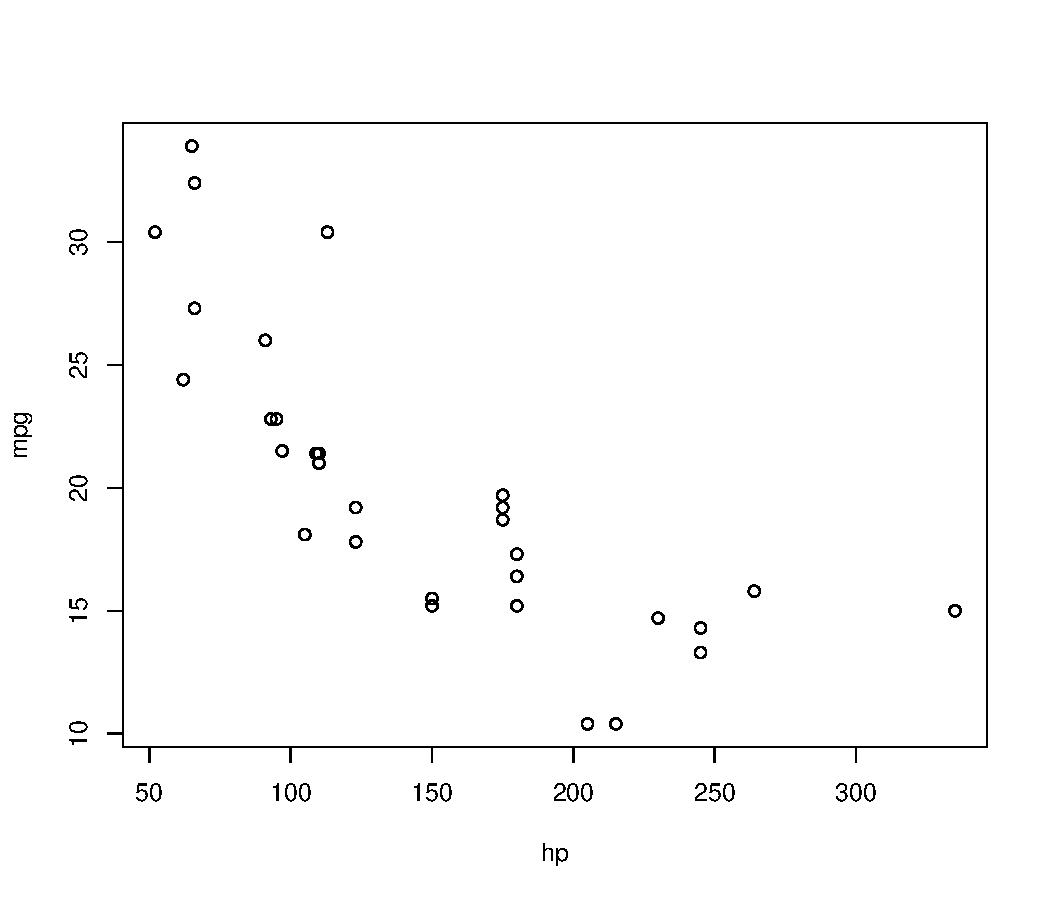
\includegraphics[width=.3\textwidth]{Project-Proposal_files/figure-latex/unnamed-chunk-2-1} 

\caption{Important scatterplot}\label{fig:unnamed-chunk-2}
\end{wrapfigure}

\hypertarget{resources}{%
\subsubsection{Resources}\label{resources}}

\hypertarget{design-and-methods-for-aim-1}{%
\subsubsection{Design and methods for Aim
1}\label{design-and-methods-for-aim-1}}

\hypertarget{design-and-methods-for-aim-2}{%
\subsubsection{Design and methods for Aim
2}\label{design-and-methods-for-aim-2}}

\hypertarget{design-and-methods-for-aim-3}{%
\subsubsection{Design and methods for Aim
3}\label{design-and-methods-for-aim-3}}

\hypertarget{timeline}{%
\subsubsection{Timeline}\label{timeline}}

There are lots of good examples of \texttt{R}-based Gantt charts to be
found by clever Googling. For displaying progress with sidebar
annotations by aim, I particularly like
\href{https://datascienceplus.com/visualize-your-cvs-timeline-with-r-gantt-style/}{\underline{this}}
example from the
\href{https://github.com/laresbernardo/lares}{\underline{lares}}
package.

\hypertarget{rigor-and-reproducibility}{%
\subsubsection{Rigor and
reproducibility}\label{rigor-and-reproducibility}}

\hypertarget{impact-of-the-proposed-study}{%
\subsubsection{Impact of the proposed
study}\label{impact-of-the-proposed-study}}

\bibliography{references.bib}


\end{document}
